%%%%%%%%%%%%%%%%%%%%%%%%%%%%%%%%%%%%%%%%%%%%%%%%%%%%%%%%%%%%%%%%%%%%%%%%%%%%%%%%%%%%%%%%%%%%%%%%%%%%%%%%%%%%%%
%                                                                                                            
%
% ------------------------------------------------------------------------------------------------------------ 
% @desc         Diploma Thesis Template for HTL St. Pölten
% ------------------------------------------------------------------------------------------------------------
%               Written by Bastian Großauer 
%
% @author       Bastian Großauer
% @datum        14.01.2022
% @file         diploma_Thesis_template.tex
%
% @depend       DA_1-4_CAPNO_nf.pdf --------------------------------------------------------------------------
%               DA_5-6_CAPNO_nf.pdf --------------------------------------------------------------------------
%               DA_7-8_CAPNO_nf.pdf --------------------------------------------------------------------------
%
% @comment      Diverse functions and packages only in LuaLaTex available
%               Therfore compile in LuaLaTeX ONLY!!!
%
%
%%%%%%%%%%%%%%%%%%%%%%%%%%%%%%%%%%%%%%%%%%%%%%%%%%%%%%%%%%%%%%%%%%%%%%%%%%%%%%%%%%%%%%%%%%%%%%%%%%%%%%%%%%%%%%               


\documentclass[12pt]{article}

% ----------------------------------------------- imports ----------------------------------------------------

\usepackage{lingmacros}
\usepackage{tree-dvips}
\usepackage{fancyhdr}
\usepackage[utf8]{inputenc}
\usepackage{fontspec}
\usepackage{graphicx}
\usepackage[document]{ragged2e}
\usepackage{xcolor}  
\usepackage{tabto}   
\usepackage{comment} 
\usepackage{pdfpages} 
\usepackage[12pt]{moresize}
\usepackage{lipsum}
\usepackage{titlesec}
\usepackage{geometry}
    \geometry{
                twoside,
                a4paper,
                total={165mm,240mm},                                                    % used text area
                left=22.5mm,                                                            % explanation: https://www.overleaf.com/learn/latex/Page_size_and_margins
                top=30mm,   
            }

\setmainfont{Arial}
\setlength{\headsep}{1.5cm}                                                             % set spce between header and section

% -------------------------------------- Page and Header/Footer Setup ------------------------------------------

\pagestyle{fancy}
\fancyhead{}
\fancyfoot{}

\setcounter{secnumdepth}{4}
\setcounter{tocdepth}{4}
\setcounter{secnumdepth}{5}
\setcounter{tocdepth}{5}

\fancyfoot[C]{}
\fancyfoot[RO, LE] {}
\renewcommand{\footrulewidth}{1pt}
\renewcommand{\headrulewidth}{1pt}

\titlespacing\section{0pt}{12pt plus 4pt minus 2pt}{0pt plus 2pt minus 2pt}
\titlespacing\subsection{0pt}{12pt plus 4pt minus 2pt}{0pt plus 2pt minus 2pt}
\titlespacing\subsubsection{0pt}{12pt plus 4pt minus 2pt}{0pt plus 2pt minus 2pt}


% ------------------------------------------- Begin of Document ------------------------------------------------

\begin{document}
%                                                                                       % not sure if there should by 1 blank or 2 in 1-4
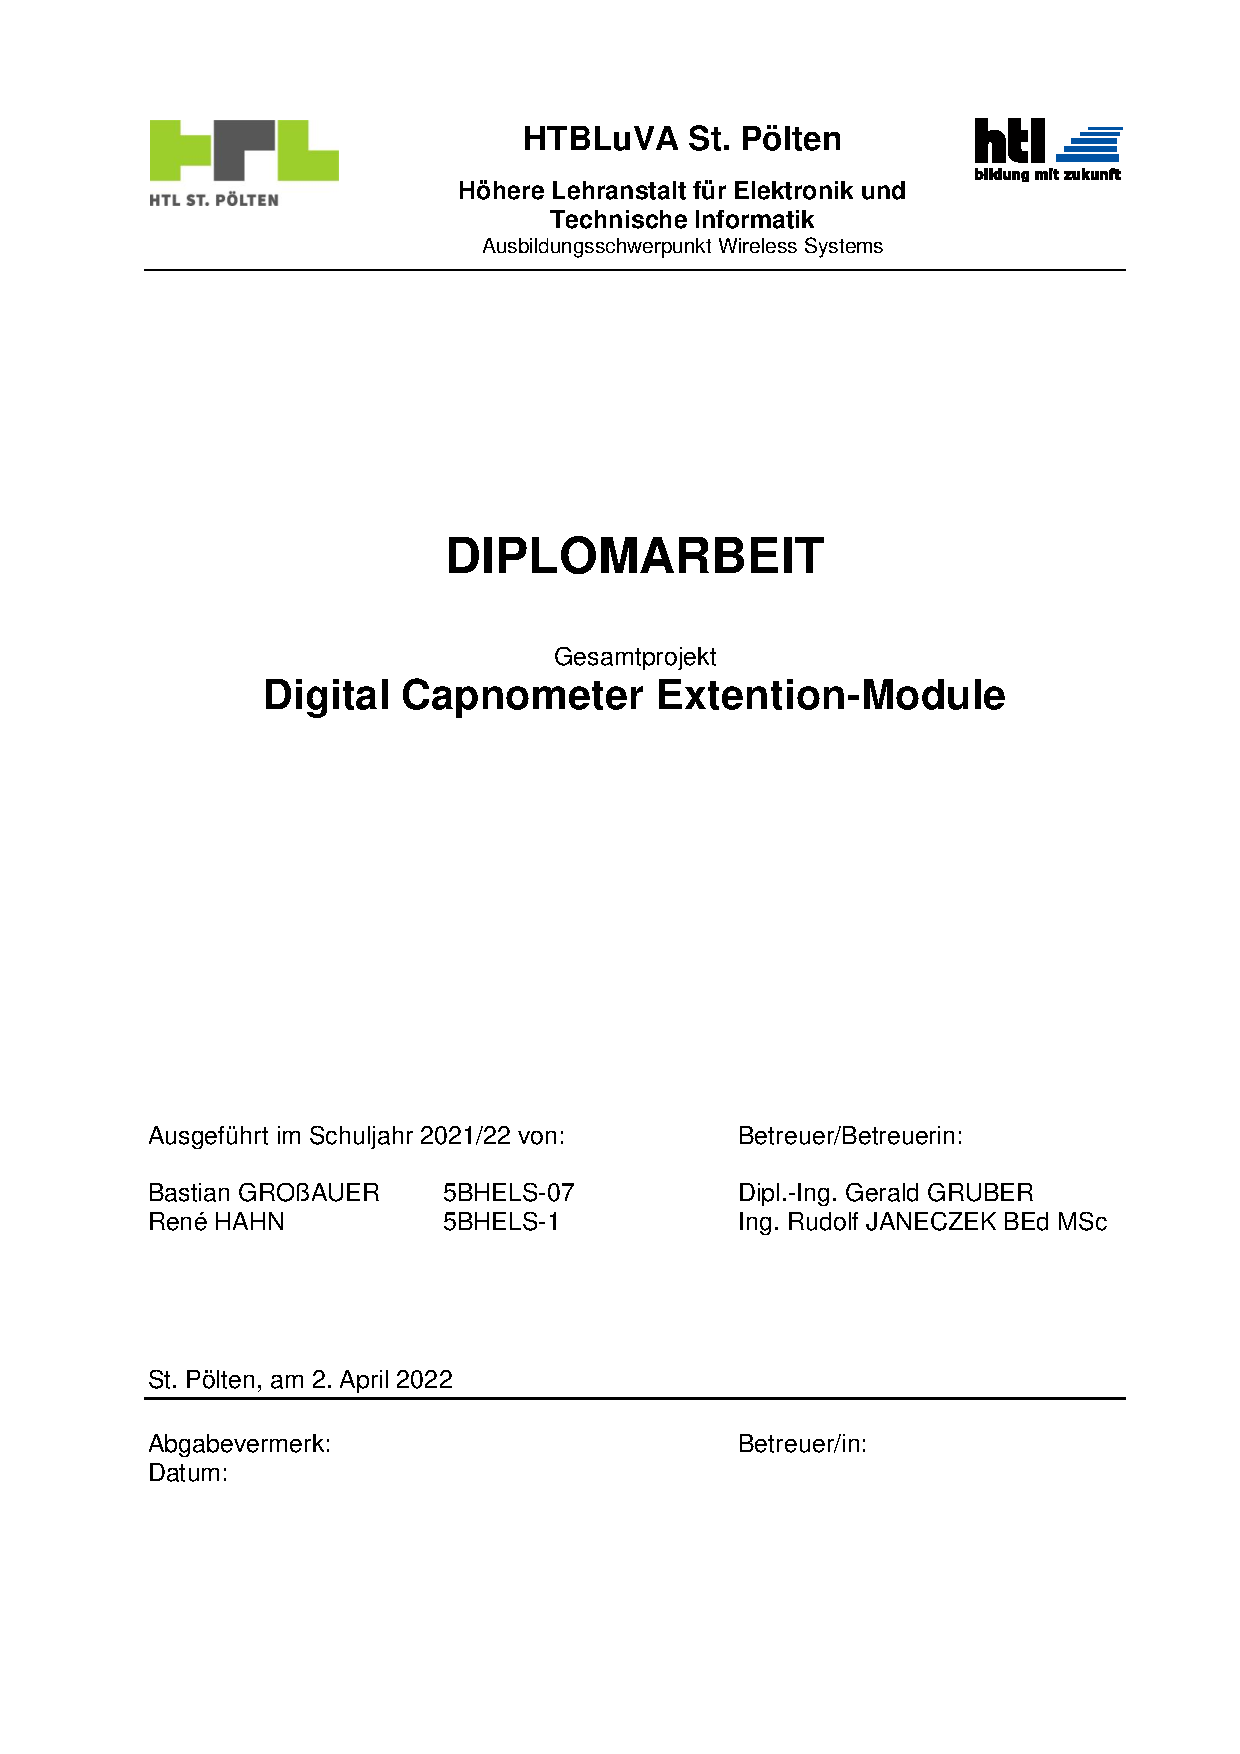
\includepdf[pages={1-4}]{./pdf/DA_1-4_CAPNO_nf.pdf}                                     % write the initial Document with the 
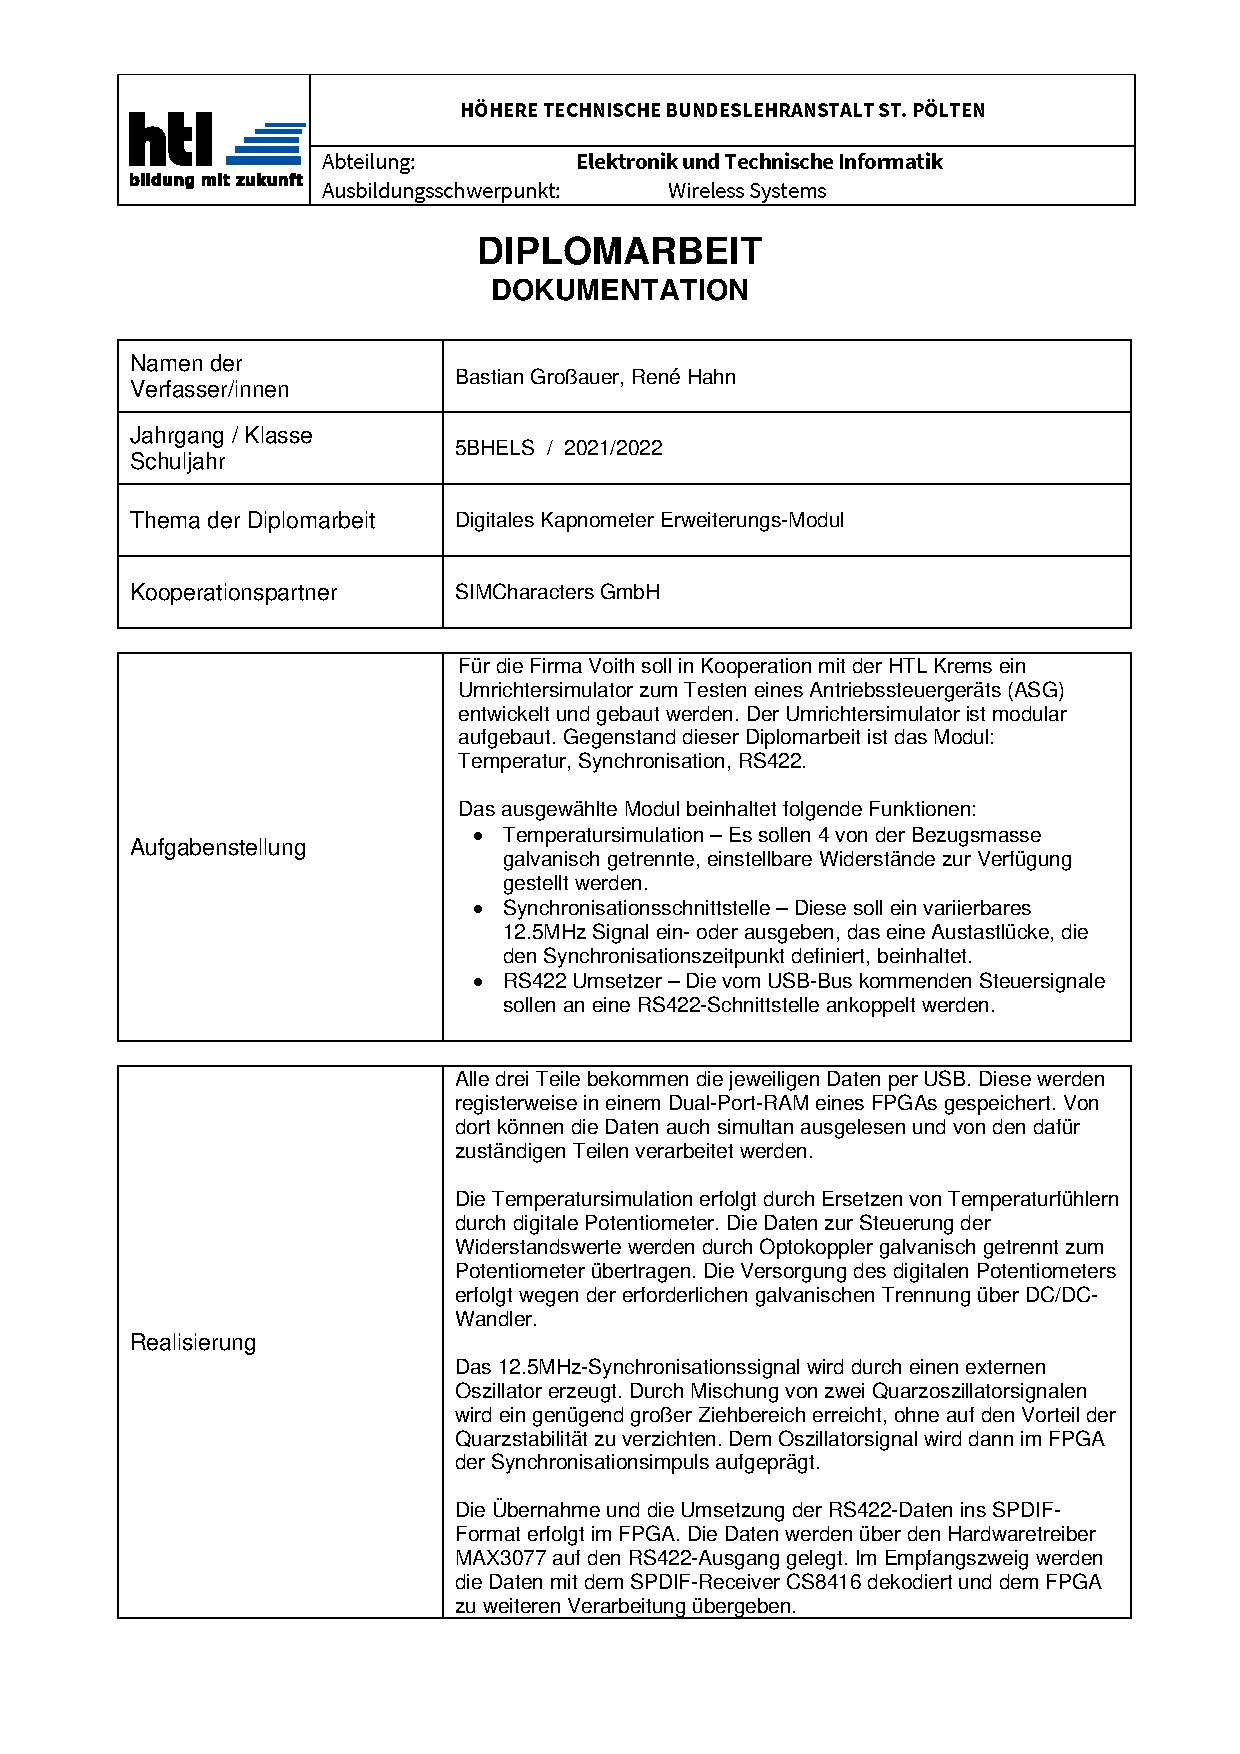
\includepdf[pages={1-2}]{./pdf/DA_5-6_CAPNO_nf.pdf}                                     % provided templates from sharepoint
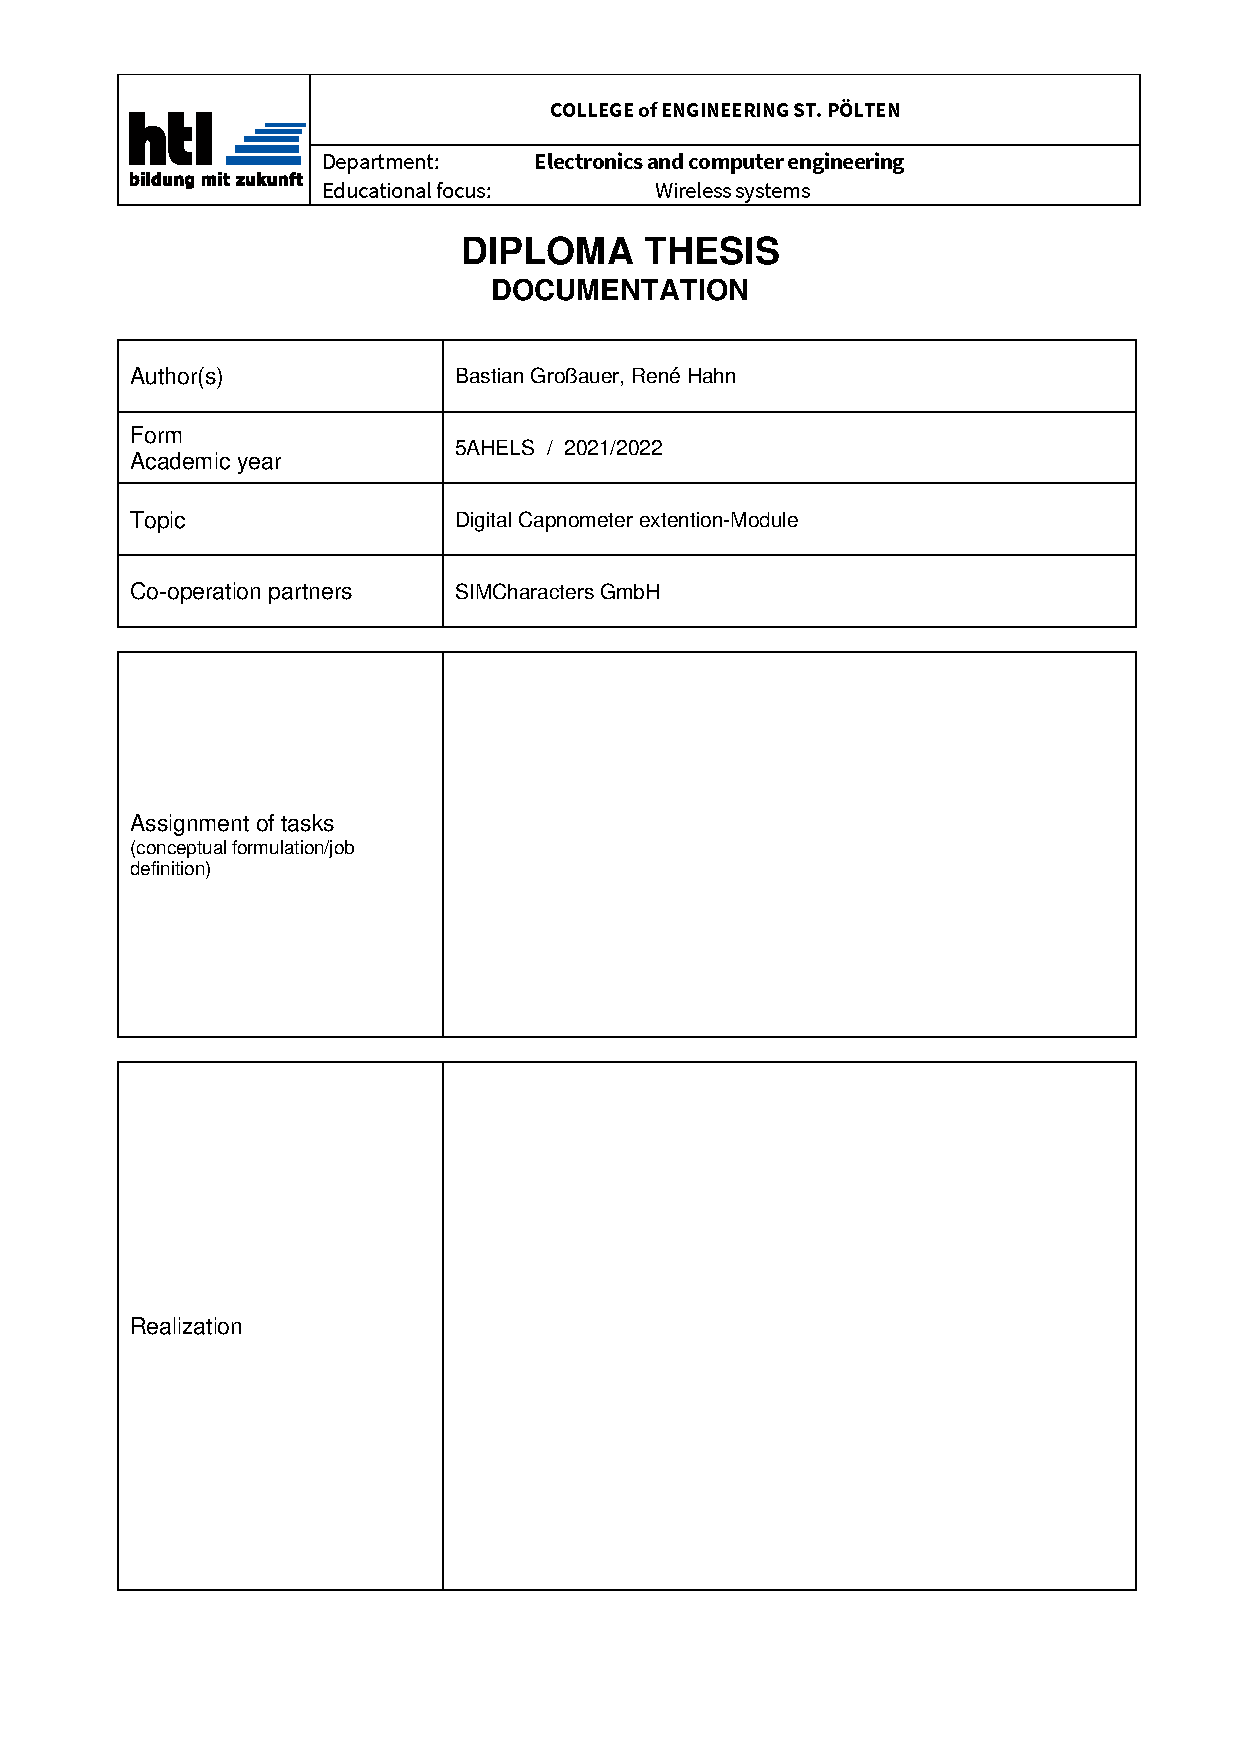
\includepdf[pages={1-2}]{./pdf/DA_7-8_CAPNO_nf.pdf}                                     % then export as pdf and add here


\fancyhead{}

\pagebreak


%  ------------------------------------------  Table of Contents-----------------------------------------------

\fancyhead{}
\fancyhead[RO,LE]{\textbf{Digital Capnometer Extention Module}\\\small{Contents}}       % change small per new section
\fancyfoot[RO,LE]{\thepage}                                                             % displaying page number on right Footer
\pagenumbering{Roman}                                                                   % set page count to roman numbers ONLY ON Table of content                                                    
\setcounter{page}{1}                                                                    %reseting page count for ToC
\tableofcontents

\pagebreak


% --------------------------------------------- actual Document ------------------------------------------------

% ---------------- Section 1 ------------------

\section{Introduction}

\fancyhead[RO,LE]{\textbf{Digital Capnometer Extention Module}\\\small{Introduction}}   % change per new section
\fancyfoot[RO,LE]{Page \thepage}    
\pagenumbering{arabic}                                                                  % set page count to roman numbers ONLY ON Table of content 
\setcounter{page}{1}

The overall goal of this ...


\subsection{Neonatology} 

The neonatology is the


\subsection{Paul as a Trainingssimulator}

Paul is a trainingssimulator for medicine students and doctors, who want to practice
an emergency case in neonatology.


\subsection{Objectives and tasks of the overall project, technical and economic environment}

The objective was to create a module, that simulates a capnometer, while communicating
with Paul.


\subsection{Individual objectives and tasks with schedule of the individual team members}

Bastian Großauer is in charge of the Hardware Design.
\fancyfoot[C]{Bastian Großauer}                                                            % change to who wrote that page, per page 

\pagebreak



% ---------------- Section 2 -------------------

\section{Basics and Methods}                                                               % Start Second Section and on ...
\fancyhead[RO,LE]{\textbf{Digital Capnometer Extention Module}\\\small{Basics and Methods}}

The overall goal of this ...


\subsection{Current Situation}

Paul is a trainingssimulator for medicine students and doctors, who want to practice
an emergency case in neonatology.


\subsubsection{Pauls Problem without the Capnometer}

The objective was to create a module, that simulates a capnometer, while communicating
with Paul.


\subsection{Possible Approaches}

The objective was to create a module, that simulates a capnometer, while communicating
with Paul.


\subsubsection{Challenges}

The objective was to create a module, that simulates a capnometer, while communicating
with Paul.


\subsubsection{Display}

The objective was to create a module, that simulates a capnometer, while communicating
with Paul.


\paragraph{Problem Factors}

The objective was to create a module, that simulates a capnometer, while communicating
with Paul.

\fancyfoot[C]{René Hahn}




\end{document}
